% Exam Template for San Jacinto Community College Math Department courses
%Copyright@Chandi Bhandari
%%%%%%%%%%%%%%%%%%%%%%%%%%%%%%%%%%%%%%%%%%%%%%%%%%%%%%%%%%%%%%%%%%%%%%%%%%%%%%%%%%%%%%%%%%%%%%

% These lines can probably stay unchanged, although you can remove the last
% two packages if you're not making pictures with tikz.
\documentclass[11pt]{exam}
\RequirePackage{amssymb, amsfonts, amsmath, latexsym, verbatim, xspace, setspace}
\RequirePackage{tikz, pgflibraryplotmarks}
\usepackage{graphicx}
\graphicspath{ {./images/} }

% By default LaTeX uses large margins.  This doesn't work well on exams; problems
% end up in the "middle" of the page, reducing the amount of space for students
% to work on them.
\usepackage[margin=1in]{geometry}


% Here's where you edit the Class, Exam, Date, etc.
\newcommand{\class}{Math 2412 Pre-Calculus}
\newcommand{\term}{Summer 2018}
\newcommand{\examnum}{Exam II}
\newcommand{\examdate}{July, 2018}
\newcommand{\timelimit}{90 Minutes}

% For an exam, single spacing is most appropriate
\singlespacing
% \onehalfspacing
% \doublespacing

% For an exam, we generally want to turn off paragraph indentation
\parindent 0ex

\begin{document} 

% These commands set up the running header on the top of the exam pages
\pagestyle{head}
\firstpageheader{}{}{}
\runningheader{\class}{\examnum\ - Page \thepage\ of \numpages}{\examdate}
\runningheadrule

\begin{flushright}
\begin{tabular}{p{3.2in} r l}
\textbf{\class} & \textbf{\term} & \textbf{\examnum}\\
\textbf{G-Number-} & \textbf{Name (Print):}  \makebox[1.2in]{\hrulefill}\\
%\textbf{Time: \timelimit} % & \makebox[2in]{\hrulefill}

\end{tabular}\\
\end{flushright}
\rule[1ex]{\textwidth}{.1pt}

\bf{ Choose Any 10 questions}

\hfill


%%%%%%%%%%%%%%%%%%%%%%%%%%%%%%%%%%%%%%%%%%%%%%%%%%%%%%%%%%%%%%%%%%%%%%%%%%%%%%%%%%%%%
%For the further information 
%%%%%%%%%%%%%%%%%%%%%%%%%%%%%%%%%%%%%%%%%%%%%%%%%%%%%%%%%%%%%%%%%%%%%%%%%%%%%%%%%%%%%

\begin{questions}

% Basic question
\addpoints
\question[10] Simplify 
\begin{parts}
\part[3] Combine the logarithm 
\begin{align*}
3ln2+2lnx-\frac{1}{2}ln(x+4)
\end{align*}
\vspace{7cm}
\part[4] Expand the logarithm
\begin{align*}
log_3\frac{\sqrt{3x^5}}{y}
\end{align*}
\vspace{7cm}
\part[3] Evaluate the logarithm
\begin{align*}
log_2 6-log_2 15 +log_2 20
\end{align*}
\end{parts}
\vspace{8cm}
% Question with parts
%\newpage
\addpoints
\question[10] 
\begin{parts}
\part[2] Express in exponential  $log_3 81=4$
\vspace{1cm}
\part[2] Express in logarithm  $10^4=10,000$
\vspace{1cm}
\part[2] Evaluate  $log_6(36)$
\vspace{1cm}.
\part[2] Find the value of x when $log_x(6)=\frac{1}{2}$
\vspace{1cm}
\part[2] Find the value of x  $log_4(x)=3$
\vspace{1cm}
\end{parts}

\newpage
\vspace{8cm}
\addpoints
\question[10] (2 point each part) Find the domain, vertical Asymptotes, Horizontal and Oblique (slant) Asymptotes (if exit), x-intercept, y-intercept of   
\begin{align*}
f(x)=\frac{\sqrt{x-2}}{x-4}
\end{align*}.

\vspace{8cm}
\addpoints
\question[10] Find Horizontal and Vertical asymptotes and Graph it $f(x)=\frac{3}{x+3}$

\newpage
\addpoints
\question[10] Graph the following

\noaddpoints % If you remove this line, the grading table will show 20 points for this problem.
\begin{parts}
	\part[5] Given the graph $log_2(x)$
	\begin{center}
		\includegraphics{log2(x).png}	
	\end{center}
	\begin{align*}
	f(x)=log_2(x-3)+2
	\end{align*}
	\begin{center}
			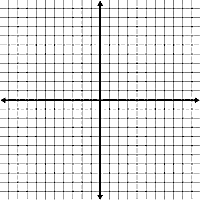
\includegraphics{graph1.png}
	\end{center}
\part[5] Graph the following function
\begin{align*}
f(x)=3^{x-3}-2
\end{align*}
\begin{center}
	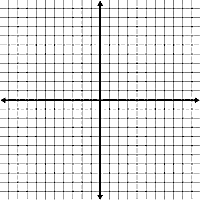
\includegraphics{graph1.png}	
\end{center}
	%\vspace{8cm}
\end{parts}
\addpoints
\question[10] Graph the following
\begin{parts}
	\part[5]  Graph
	\[f(x)=\frac{x^3-2x^2}{x-2}	\]
\begin{center}
	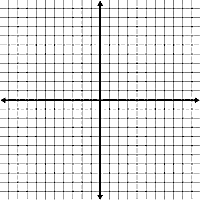
\includegraphics{graph1.png}	
\end{center}
\vspace{2cm}
\part[5]  Graph
\[f(x)=\frac{x-3}{x^2-3x}	\]
\begin{center}
	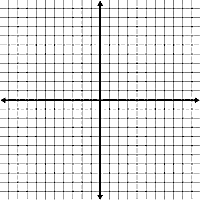
\includegraphics{graph1.png}	
\end{center}
\end{parts}



\addpoints
\question[10] (2 points each)For the given quadratic function 
\begin{align*}
f(x)=x^2-2x+3
\end{align*}
\begin{parts}
\part Express in standard form 
\part Find Vertex
\part Find X-intercept, Y-intercept
\part Sketch the graph 
\part Find the domain and range
\end{parts}

\vspace{8cm}
\addpoints
\question[10] If \$600 is invested at an interest rate of 2.5\% per year, find the amount of the investment at the end of 10 years for the quarterly compounding methods.

\vspace{8cm}
\addpoints
\question[10] Find the quotient and remainder by using the Synthetic division for 
\begin{align*}
\frac{x^5+3x^3-6}{x-1}
\end{align*}

\vspace{10cm}
\addpoints
\question[10] Find the quotient and remainder by using the long division for 
\begin{align*}
\frac{x^3+3x^2+4x+3}{3x+6}
\end{align*}


\vspace{8cm}
\addpoints
\question[10] Check that whether x+2 is the factor of the polynomial $P(x)=x^3+2x^2-7$, why or why not give a reason. Use the remainder theorem to compute the remainder. 


\vspace{8cm}
\noaddpoints
\question[5 Bonus] Write down all the possible rational solution of $P(x)=2x^3+2x^2-24$, Use Descrates Rules to determine how many positive and negative solution does it have?
 


\end{questions}
\end{document}